\documentclass{beamer}
%\documentclass[UTF8]{ctexbeamer} % Chines Version

\usepackage[utf8]{inputenc}
\usepackage{utopia}            % font utopia imported
\usepackage{amsmath}
\usepackage{latexsym}
\usepackage{calc}              % support command '\widthof'
\usepackage{xcolor}            % support multiple color 
\usepackage{arydshln}
\usepackage{amssymb}  
\usepackage{booktabs}
\usepackage{graphicx}
\usepackage{subcaption}
\usepackage{bookmark}
\usepackage{float}
\usepackage{bm}
\usepackage{bbold}
\usepackage{extarrows}

%--------
\usepackage{listings}
\usepackage{xcolor}

\usefonttheme{professionalfonts} 

\makeatletter
\let\@@magyar@captionfix\relax
\makeatother

\usetheme{Madrid}
%\usetheme{Singapore}
%\usetheme{Pittsburgh}
%\usecolortheme{default,beaver,lily,orchid,seahorse} 
\usecolortheme{default}
%default、albatross、beaver、beetle、crane、dolphine、dove、fly、lily、orchid、rose、seagull、seahorse、sidebartab、structure、whale、wolverine

%======================================================================%
\title[CMT.SCNU]{High-temperature topological superconductivity in twisted double layer copper oxides}

%\subtitle{(To throw out a brick to attract a jade)}

\author[YuXuan Li]
{YuXuan Li\inst{1}}  

\institute[Physics@SCNU] 
{
  \inst{1}%
  Department of Physics\\
 South China Normal University 
}

\date[SCNU]{22.Dec.2020}
%======================================================================

%======================================================================
\AtBeginSection[]
{
  \begin{frame}
    \frametitle{Outline}
    \tableofcontents[currentsection]
  \end{frame} 
}
%======================================================================
 
\begin{document}
  %======================================================================
  \frame{\titlepage}
  %======================================================================

  %======================================================================
  \begin{frame}
    \frametitle{Outline}
    \tableofcontents
  \end{frame}
%======================================================================
\section{Pairing Symmetry}
\begin{frame}
\frametitle{D-orbit of Hydrogen}
\begin{figure}[h]
	\centering
	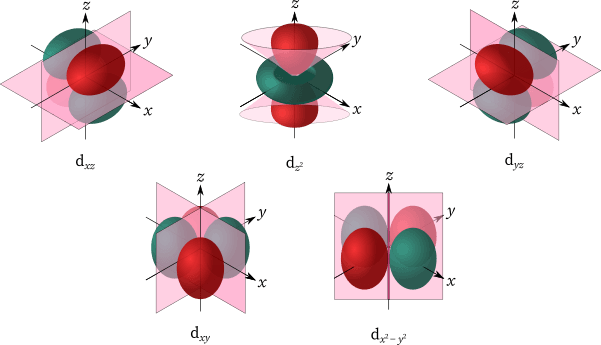
\includegraphics[scale=0.4]{pic/p2.png}
\end{figure}
%------------------------------------
\begin{equation}
\Delta(\mathbf{k})=\Delta_0(\cos k_x-\cos k_y)
\end{equation}
\end{frame}
%----------------------------------------------------------
\begin{frame}
\frametitle{Twisted double layer copper-oxygen square
	lattices\footnote{Nature,575,156}}
\begin{figure}
\centering
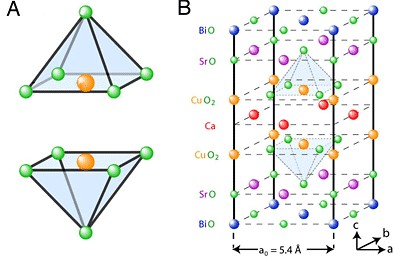
\includegraphics[scale=0.6]{pic/p3.png}
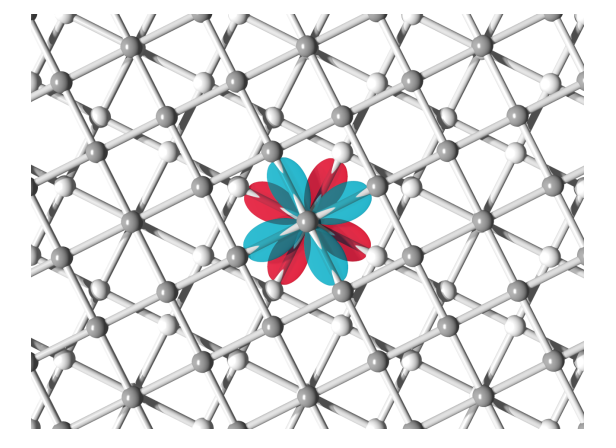
\includegraphics[scale=0.4]{pic/p1.png}
\end{figure}
\begin{equation}
\Delta_\mathbf{k}^\theta=\Delta_0\left[\cos(2\theta)(\hat{k_x^2}-\hat{k_y^2})+\sin(2\theta)2\hat{k_x}\hat{k_y}\right]\label{eq1}
\end{equation}
The second term in Eq.(\ref{eq1}) has the functional form of a $d_{xy}$ order parameter.
\end{frame}
%--------------------------------------------------------------------
\begin{frame}
\frametitle{Twisted double layer copper-oxygen square lattices}
\begin{figure}[h]
\centering
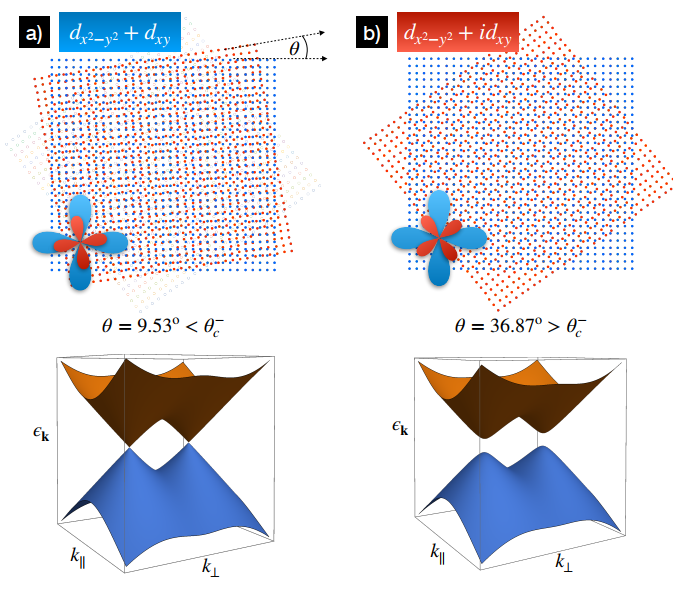
\includegraphics[scale=0.4]{pic/p4.png}
\end{figure}
$T$-breaking is evident because time reversal maps $d+id'$ to $d-id'$.
\end{frame}
%========================================================================================
\section{Ginzburg Landau(GL) theory}
\begin{frame}
\frametitle{GL Free Energy Density }
\begin{equation}
|\psi(\mathbf{r})|^2=n_s(\mathbf{r})
\end{equation}
\begin{equation}
f_s=f_n+\alpha(T)n_s+\frac{1}{2}\beta(T)n_s^2+\cdots
\end{equation}
\begin{equation}
f_s=f_n+\alpha(T)|\psi(\mathbf{r})|^2+\frac{1}{2}\beta(T)|\psi(\mathbf{r})|^4
\end{equation}
\end{frame}
%----------------------------------------------------------------------------------------
\begin{frame}
\frametitle{GL Free Energy Density}
\begin{equation}
\mathcal{F}\left[\psi_1,\psi_2\right]=f_0\left[\psi_1\right]+f_0\left[\psi_2\right]+A|\psi_1|^2|\psi_2|^2+B(\psi_1\psi_2^*+c.c)+C(\psi_1^2\psi_2^{*2}+c.c)\label{eq2}
\end{equation}
where $\psi_{a=1,2}$ are complex order parameters of two layers and $f_0\left[\psi\right]=\alpha|\psi|^2+\frac{1}{2}\beta|\psi|^4$ is the free energy of
a monolayer.

If the two layers are physically identical, then the order parameter amplitudes must be the same and the most general
solution (up to an overall phase) is
\begin{equation}
\psi_1=\psi\qquad\psi_2=\psi e^{i\varphi}
\end{equation}
\begin{equation}
\psi_a\rightarrow -\psi_a\quad\textrm{Under rotation}\quad 90^\circ
\end{equation}
For the free energy $(\ref{eq2})$ to remain invariant, the parameter $B$ must also change sign
\begin{equation}
B=-B_0\cos(2\theta)
\end{equation}
\end{frame}
%--------------------------------------------------------------------
\begin{frame}
\frametitle{GL Free Energy Density}
\begin{equation}
\mathcal{F}(\varphi)=\mathcal{F}_0+2B_0\psi^2\left[-\cos(2\theta)\cos\varphi+\mathcal{K}\cos(2\varphi)\right]
\end{equation}
where $\mathcal{K}=C\psi^2/B_0$ and $\mathcal{F}_0$ contains all terms independent of $\varphi$.
\begin{figure}
\centering
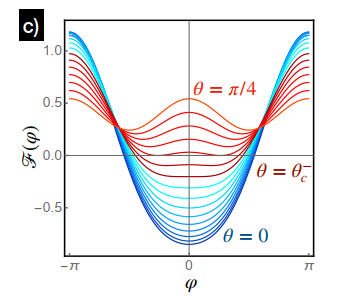
\includegraphics[scale=0.5]{pic/p5.png}
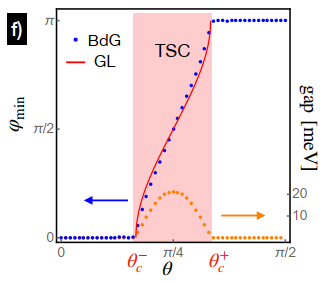
\includegraphics[scale=0.5]{pic/p6.png}
\end{figure}
For $\theta\neq 45^\circ$, the free energy is minimized by
\begin{equation}
\varphi_{\textrm{min}}=\arccos(\frac{\cos 2\theta}{4\mathcal{K}})
\end{equation}
\end{frame}
%----------------------------------------------------------------
\begin{frame}
\frametitle{GL Theory}
Temperature dependence for the order parameter $\psi(T)=\psi_0\sqrt{1-T/T_c}$, we can obtain
\begin{equation}
\tilde{T_c}(\theta)=T_c(1-\frac{|\cos 2\theta|}{4\mathcal{K}_0})\quad\theta^{-}_c\le\theta\le\theta^{+}_c
\end{equation}
where $\mathcal{K}_0=C\psi_0^2/B_0$. 
\begin{figure}
\centering
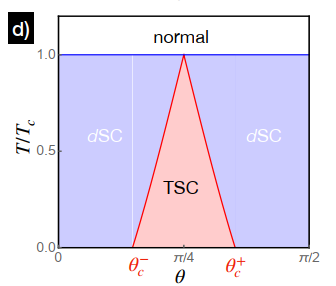
\includegraphics[scale=0.5]{pic/p7.png}
\end{figure}
\end{frame}
%=============================================================================
\section{Microscopic Theory}
\begin{frame}
\frametitle{Microscopic Theory}
\begin{equation}
\begin{aligned}
\mathcal{H}&=\sum_{\mathbf{k}\sigma a}\xi_{\mathbf{k}a}c^\dagger_{\mathbf{k}\sigma a}c_{\mathbf{k}\sigma a}+g\sum_{\mathbf{k}\sigma}(c^\dagger_{\mathbf{k}\sigma 1}c_{\mathbf{k}\sigma 2}+h.c)\\
&+\sum_{\mathbf{k}a}(\Delta_{\mathbf{k}a}c^\dagger_{\mathbf{k}\uparrow a}c^\dagger_{-\mathbf{k}\downarrow a}+h.c)-\sum_{\mathbf{k}a}\Delta_{\mathbf{k}a}\langle c^\dagger_{\mathbf{k}\uparrow a}c^\dagger_{-\mathbf{k}\downarrow a}\rangle
\end{aligned}
\end{equation}
%------------------------
\begin{equation}
\Delta_{\mathbf{k}a}=\sum_\mathbf{p}^{'}V_\mathbf{kp}^{(a)}\langle c_{-\mathbf{p}\downarrow a}c_{\mathbf{p}\uparrow a} \rangle
\end{equation}
where $V^{(a)}_{\mathbf{kp}}$ denotes the interaction matrix element in layer a.
\begin{equation}
V^{(a)}_\mathbf{kp}=-2\mathcal{V}\cos(2\alpha_\mathbf{k})\cos(2\alpha_\mathbf{p})
\end{equation}
where $\alpha_\mathbf{k}$ represents the polar angle of the vector $\mathbf{k}$. 
\end{frame}
%------------------------------------
\begin{frame}
\frametitle{Microscopic Theory}
Rotate the interaction in layer 2 by angle $\theta$
\begin{equation}
V^{(2)}_\mathbf{kp}=-2\mathcal{V}\cos(2\alpha_\mathbf{k}-2\theta)\cos(2\alpha_\mathbf{p}-2\theta)
\end{equation}
Consider a circular Fermi surface generated by $\xi_{\mathbf{k}a}=\hbar^2k^2/2m-\mu$ that remains invariant under rotation	
\begin{figure}
\centering
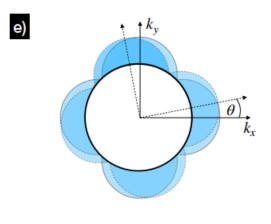
\includegraphics[scale=0.6]{pic/p8.png}
\end{figure}
\begin{equation}
\mathcal{H}=\sum_\mathbf{k}\Psi^\dagger_\mathbf{k}h_\mathbf{k}\Psi_\mathbf{k}+E_0
\end{equation}
\end{frame}
%---------------------------------------------------------
\begin{frame}
\frametitle{Microscopic Theory}
\begin{equation}
h_\mathbf{k}=\left[
\begin{array}{cccc}
\xi_\mathbf{k}&\Delta_{\mathbf{k}1}&g&0\\
\Delta_{\mathbf{k}1}^*&-\xi_\mathbf{k}&0&-g\\
g&0&\xi_\mathbf{k}&\Delta_{\mathbf{k}2}\\
0&-g&\Delta_{\mathbf{k}2}^*&-\xi_\mathbf{k}
\end{array}
\right]
\end{equation}
and $E_0=\sum_\mathbf{k}2\xi_\mathbf{k}-\sum_{\mathbf{k}a}\Delta_{\mathbf{k}a}\langle c^\dagger_{\mathbf{k}\uparrow a}c^\dagger_{-\mathbf{k}\downarrow a} \rangle$.

The free energy of the system
can be calculated from the standard expression
\begin{equation}
\mathcal{F}_{\mathrm{BdG}}=E_0-2k_BT\sum_{\mathbf{k}a}\ln \left[2\cosh(E_{\mathbf{k}\alpha}/2k_BT)\right]
\end{equation}
\begin{equation}
\begin{aligned}
E_{\mathbf{k}\alpha}&=\sqrt{(\Delta^2_{\mathbf{k}1}+\Delta^2_{\mathbf{k}2})/2+\xi^2_{\mathbf{k}}+g^2+(-)^\alpha D_\mathbf{k}}\\
D^2_\mathbf{k}&=(D^2_{\mathbf{k}1}-D^2_{\mathbf{k}2})^2/4+g^2(\Delta^2_{\mathbf{k}1}+\Delta^2_{\mathbf{k}2}+4\xi^2_\mathbf{k})-2g^2\Delta_{\mathbf{k}1}\Delta_{\mathbf{k}2}\cos\varphi
\end{aligned}
\end{equation}
\end{frame}
%---------------------------------------------------------
\begin{frame}
\frametitle{Microscopic Theory}
\begin{equation}
\Delta_{\mathbf{k}1}=\psi\cos(2\alpha_\mathbf{k})\qquad \Delta_{\mathbf{k}2}=\psi\cos(2\alpha_\mathbf{k}-2\theta)
\end{equation}
\begin{equation}
\mathcal{F}(\varphi)=\mathcal{F}_0+2B_0\psi^2\left[-\cos(2\theta)\cos\varphi+\mathcal{K}\cos(2\varphi)\right]
\end{equation}
\begin{figure}
\centering
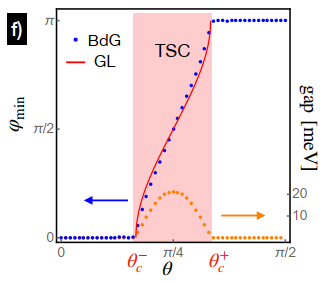
\includegraphics[scale=0.8]{pic/p6.png}
\end{figure}
\end{frame}
%=========================================================
\section{Lattice Model}
\begin{frame}
\frametitle{Hubbard Model}
\begin{figure}
\centering
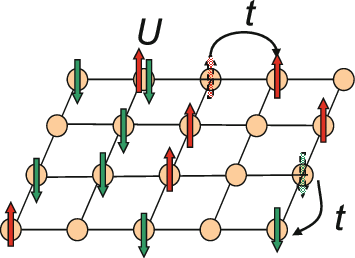
\includegraphics[scale=0.5]{pic/p13.png}
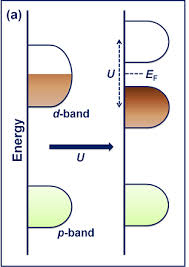
\includegraphics[scale=0.5]{pic/p14.jpg}
\end{figure}
\begin{equation}
H=\sum_{ij,\sigma}t_{ij}C^\dagger_{i\sigma}C_{j\sigma}+U\sum_{i\sigma}n_{i\sigma}n_{i\bar{\sigma}}\qquad n_{i\sigma}=C^\dagger_{i\sigma}C_{i\sigma}
\end{equation}
\end{frame}
%-------------------------------------------------
\begin{frame}
\frametitle{Hubbard Model}
\begin{equation}
H=-\sum_{ij,\sigma a}t_{ij}c^\dagger_{i\sigma a}c_{j\sigma a}-\mu\sum_{i\sigma a}n_{i\sigma a}+\textcolor{blue}{\sum_{ij,a}V_{ij}n_{ia}n_{ja}}-\sum_{ij\sigma}g_{ij}c^\dagger_{i\sigma 1}c_{j\sigma 2}
\end{equation}
Mean field approximation
\begin{equation}
c_ic_j=\langle c_ic_j\rangle+(c_ic_j-\langle c_ic_j\rangle)
\end{equation}
%------------------------------------------
\begin{equation}
\begin{aligned}
H&=-t\sum_{\langle ij\rangle\sigma a}c^\dagger_{i\sigma a}c_{j\sigma a}-t^{'}\sum_{\langle\langle ij\rangle\rangle\sigma a}c^\dagger_{i\sigma a}c_{j\sigma a}-\mu\sum_{i\sigma a}n_{i\sigma a}\\
&+\sum_{\langle ij\rangle a}(\Delta_{ij,a}c^\dagger_{i\uparrow a}c^\dagger_{j\downarrow a}+h.c)-\sum_{ij\sigma}g_{ij}c^\dagger_{i\sigma 1}c_{j\sigma 2}\label{eq3}
\end{aligned}
\end{equation}
\begin{equation}
\Delta_{ij,a}=V\langle c_{i\uparrow a}c_{j\downarrow a}\rangle
\end{equation}
\end{frame}
%--------------------------------------------------------
\begin{frame}
\frametitle{Hubbard-Stratonovich Transformation\footnote{Condensed Matter Field Theory(Alexander Altland,Ben Simons)}}
\begin{equation}
S\left[\psi,\bar{\psi}\right]=\sum_p\bar{\psi}_{p\sigma}(-i\omega_n+\frac{p^2}{2m}-\mu)\psi_{p\sigma}+\textcolor{blue}{\frac{T}{2L^3}\sum_{pp'q}\bar{\psi}_{p+q\sigma}\bar{\psi}_{p'-q\sigma'}V(\mathbf{q})\psi_{p'\sigma}\psi_{p\sigma}}
\end{equation}
\begin{equation}
1\equiv\int D\phi \mathrm{exp}\left[-\frac{e^2\beta}{2L^d}\sum_q\phi_q V^{-1}(\mathbf{q})\phi_{-q} \right]
\end{equation}
Employing the variable shift $\phi_q\rightarrow \phi_q+ie^{-1}V(q)\rho_q/\beta$, where $\rho_q\equiv\sum_p\bar{\psi}_{p\sigma}\psi_{p+q\sigma}$, $q=(\omega_m,\mathbf{q})$.
\begin{equation}
1=\int D\phi \textrm{exp}\left[\frac{1}{L^d}\sum_q(-\frac{e^2\beta}{2}\phi_qV^{-1}(q)\phi_{-q}+ie\rho_q\phi_{-q}+\textcolor{blue}{\frac{1}{2\beta}\rho_qV(\mathbf{q})\rho_{-q}}) \right]
\end{equation}
\end{frame}
%-------------------------------------------------------------------------------
\begin{frame}
\frametitle{Hubbard-Stratonovich Transformation}
The field integral 
\begin{equation}
\mathcal{Z}=\int D\phi\int \textcolor{blue}{D(\bar{\psi}_\sigma,\psi_\sigma)}e^{-S\left[\phi,\bar{\psi}_\sigma,\psi_\sigma\right]}
\end{equation}

\begin{equation}
\begin{aligned}
S\left[\phi,\bar{\psi}_\sigma,\psi_\sigma\right]=&\frac{\beta}{8\pi L^d}\sum_q\phi_q\mathbf{q}^2\phi_{-q}\\
&+\sum_{pp'}\bar{\psi}_{p\sigma}\left[(-i\omega+\frac{\mathbf{p}}{2m}-\mu)\delta_{pp'}+\frac{ie}{L^d}\phi_{p'-p}\right]\psi_{p'\sigma}
\end{aligned}
\end{equation}
\end{frame}
%-------------------------------------------------------------------------------
\begin{frame}
\frametitle{Hubbard-Stratonovich Transformation}
After decoupling the attractive pairing potential in the
Cooper channel with the Hubbard-Stratonovich transformation we obtain the action corresponding to the Hamiltonian $(\ref{eq3})$
\begin{equation}
S=\sum_{\mathbf{k}n}\Psi^\dagger_{\mathbf{k}n}\left[-i\omega_n+h_\mathbf{k}\right]\Psi_{\mathbf{k}n}+\frac{\beta \mathcal{N}}{V}\sum_{i,j\in u.c.a}\Delta_{ij,a}\Delta^*_{ij,a}
\end{equation}
The effective action for $\Delta_{ij,a}$ can be determined by integrating out fermionic degrees of freedom 
\begin{equation}
S_{\mathrm{eff}}=-\sum_{\mathbf{k}n}\mathrm{Tr}\log\left[-\mathcal{G}(\mathbf{k},i\omega)^{-1}\right]+\frac{\beta \mathcal{N}}{V}\sum_{i,j\in u.c.a}\Delta_{ij,a}\Delta^*_{ij,a}
\end{equation}
where $\mathcal{G}(\mathbf{k},i\omega_n)=-(-i\omega_n+h_\mathbf{k})^{-1}$
\end{frame}
%-------------------------------------------------------------------------------
\begin{frame}
\frametitle{Hubbard-Stratonovich Transformation}
Calculate the saddle point condition for this effective action $\partial S_{\mathrm{eff}}/\partial\delta^*_{ij,a}=0$, employ the identity $\partial_\Delta(\mathrm{Tr}\log A)=\mathrm{Tr}\left[\partial_\Delta AA^{-1}  \right]$. After performing the Matsubara sum
\begin{equation}
\Delta_{ij,a}=-\frac{V}{\mathcal{N}}\sum_\mathbf{k}\mathrm{Tr}\left[\frac{\partial h_\mathbf{k}}{\partial \Delta^*_{ij,a}}U_\mathbf{k}n_F(E_\mathbf{k})U^\dagger_\mathbf{k}\right]
\end{equation}
where $U^\dagger_\mathbf{k}h_\mathbf{k}U_\mathbf{k}=E_\mathbf{k}$ and $n_F(E_\mathbf{k})$ is Fermi function.
\end{frame}
%-------------------------------------------------------------------------------
\begin{frame}
\frametitle{Hubbard Model}
\begin{figure}
\centering
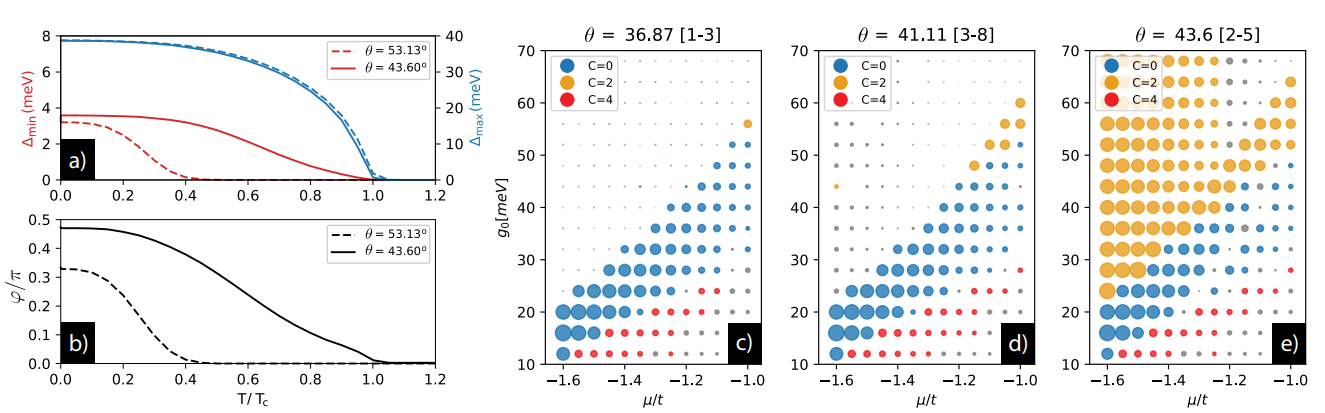
\includegraphics[scale=0.5]{pic/p9.png}
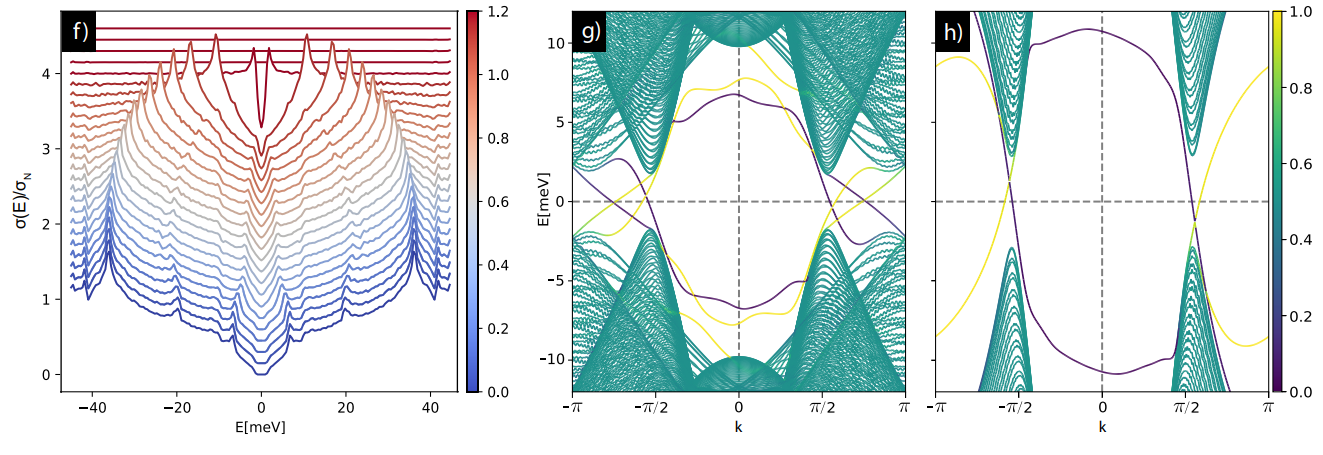
\includegraphics[scale=0.5]{pic/p10.png}
\end{figure}
\end{frame}
%==================================================================================================================
\section{Topological Phase}
\begin{frame}
\frametitle{Chern Number}
\begin{equation}
C=\frac{1}{2\pi}\int_{BZ}\Omega(\mathbf{k})d^2k
\end{equation}
\begin{equation}
\Omega(\mathbf{k})=\sum_{m\neq n}\frac{\langle n|\nabla_\mathbf{k}h_\mathbf{k}|m\rangle\times\langle m|\nabla_\mathbf{k}h_\mathbf{k}|n\rangle}{(E_m-E_n)^2}
\end{equation}
\begin{figure}
\centering
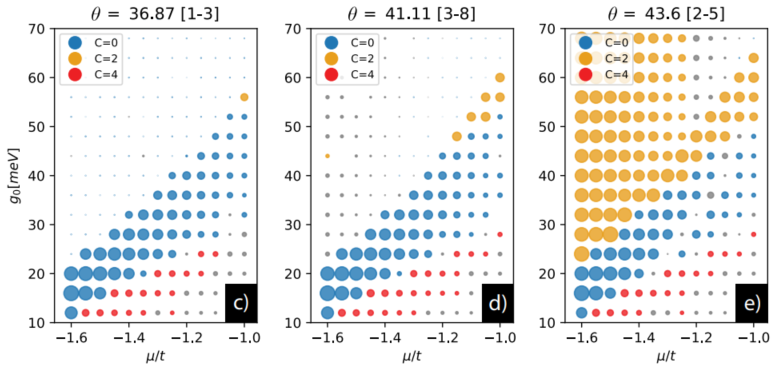
\includegraphics[scale=0.5]{pic/p11.png}
\end{figure}
\end{frame}
%---------------------------------------------------------
\begin{frame}
\frametitle{$d$-wave Superconductor}
\begin{equation}
H=\sum_{\mathbf{k}\sigma}\epsilon(\mathbf{k})d^\dagger_{\mathbf{k}\sigma}d_{\mathbf{k}\sigma}+\sum_{\mathbf{k}}\Delta(\mathbf{k})(d^\dagger_{\mathbf{k}\uparrow}d^\dagger_{\mathbf{-k}\downarrow}+h.c)
\end{equation}
where $\epsilon(\mathbf{k})=-2t(\cos k_x+\cos k_y)-\mu$, $\Delta(\mathbf{k})=\Delta_0(\cos k_x-\cos k_y)$
\begin{figure}
\centering
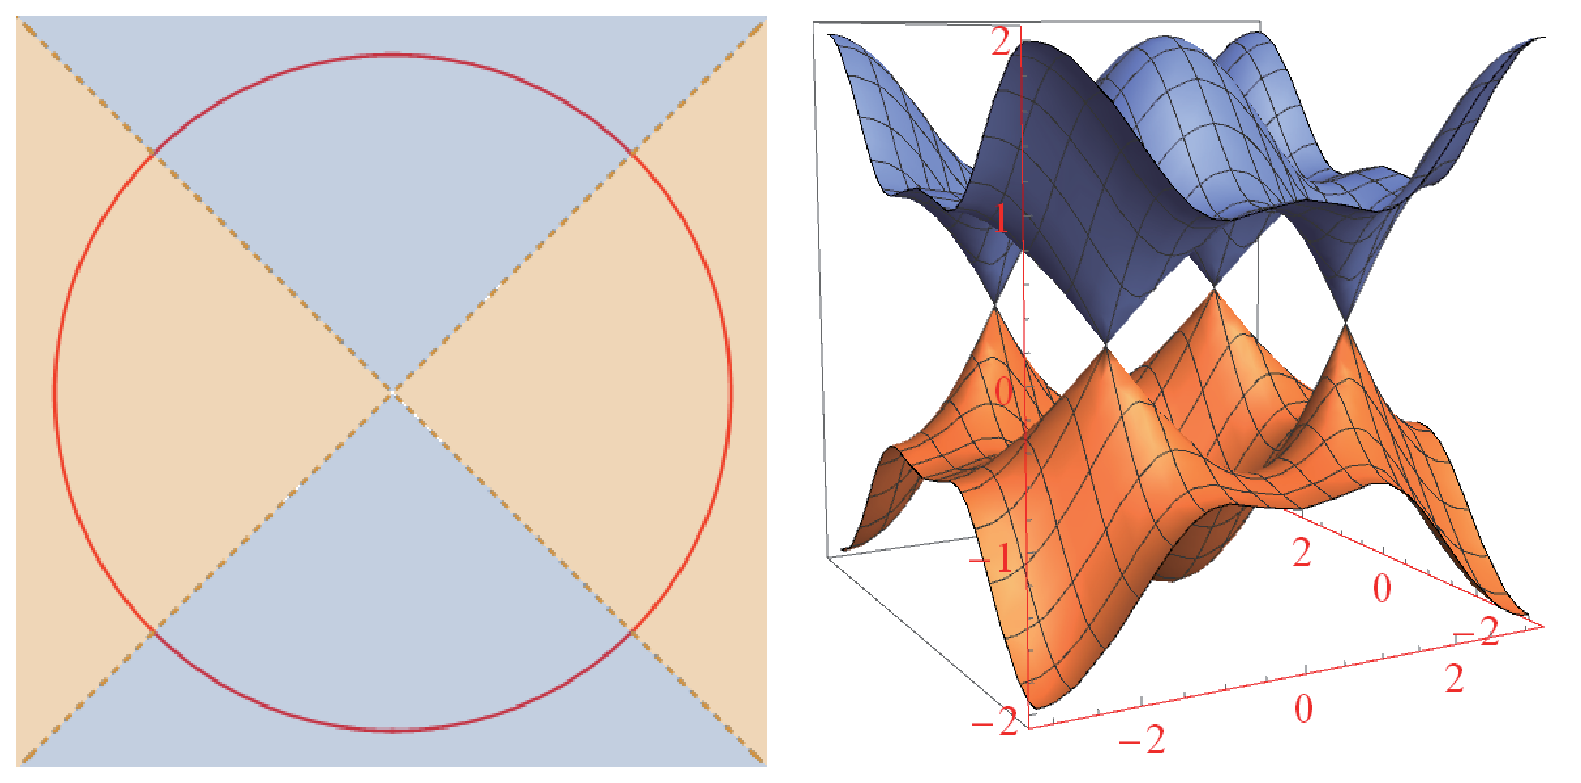
\includegraphics[scale=0.25]{pic/p15.eps}
\end{figure}
\end{frame}
%---------------------------------------------------------
\begin{frame}
\frametitle{Chern Number}
\begin{figure}
\centering
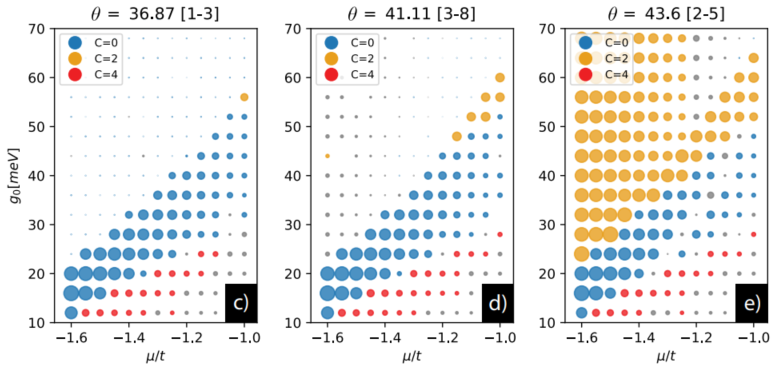
\includegraphics[scale=0.4]{pic/p11.png}
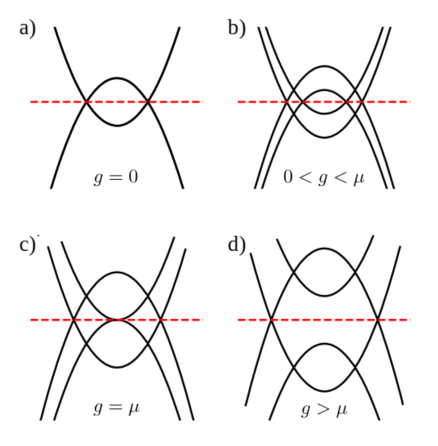
\includegraphics[scale=0.5]{pic/p12.png}
\end{figure}
\begin{block}{}
If the interlayer coupling g is strong
enough to push one of the bands above the Fermi level,
half of the Dirac cones disappear, leaving four Dirac cones behind.
\end{block}
\end{frame}
%==========================================================================
\section{Experiment}
\begin{frame}
\frametitle{Van der Waals heterostructures\footnote{Nature,499,419-425(2013)}}
\begin{figure}
\centering
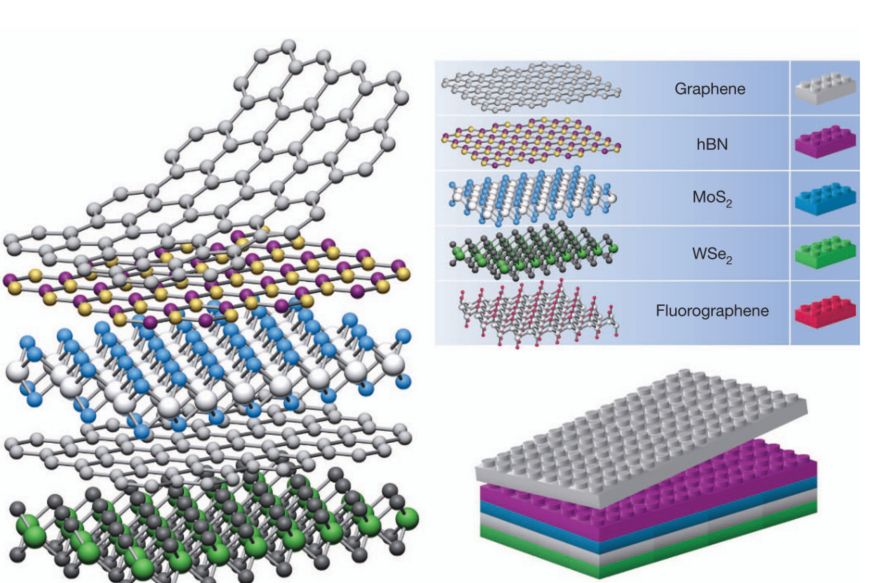
\includegraphics[scale=0.5]{pic/p17.png}
\end{figure}
\end{frame}
%------------------------------------------------------------------
\begin{frame}
\frametitle{Topological superconductivity\footnote{Nature,588,424-428(2020)}}
\begin{figure}
\centering
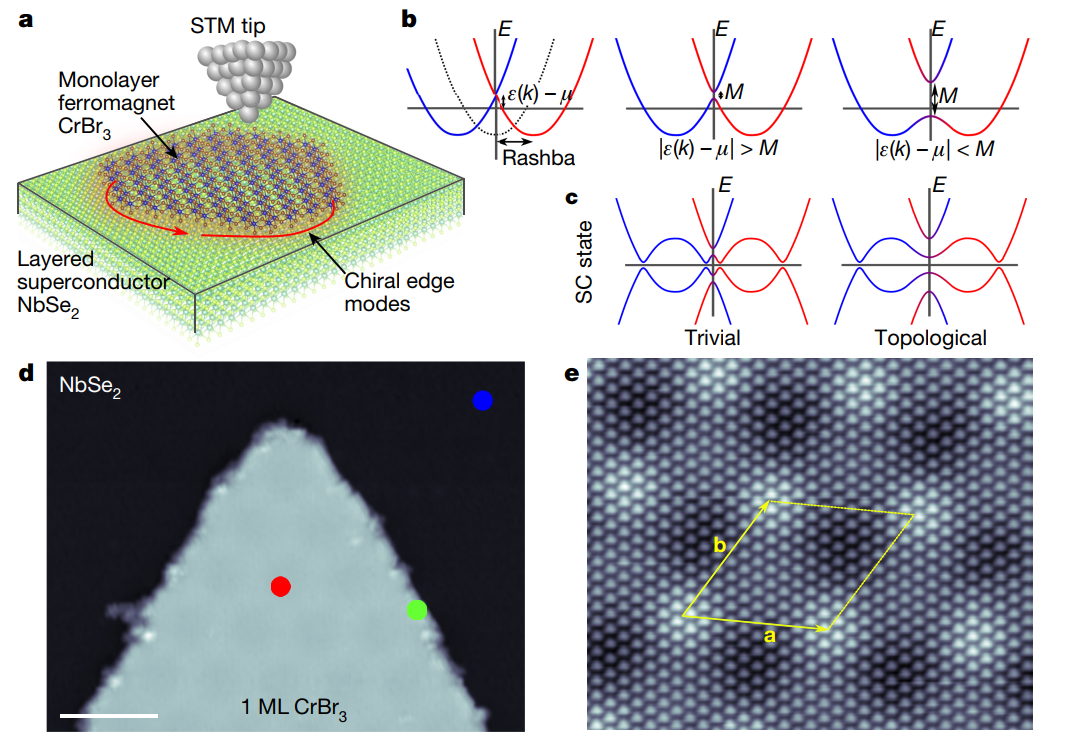
\includegraphics[scale=0.5]{pic/p18.png}
\end{figure}
\end{frame}
%-----------------------------------------------------------------
\begin{frame}
\frametitle{Quantum anomalous Hall insulators\footnote{Nature,588,419-423(2020)}}
\begin{figure}
\centering
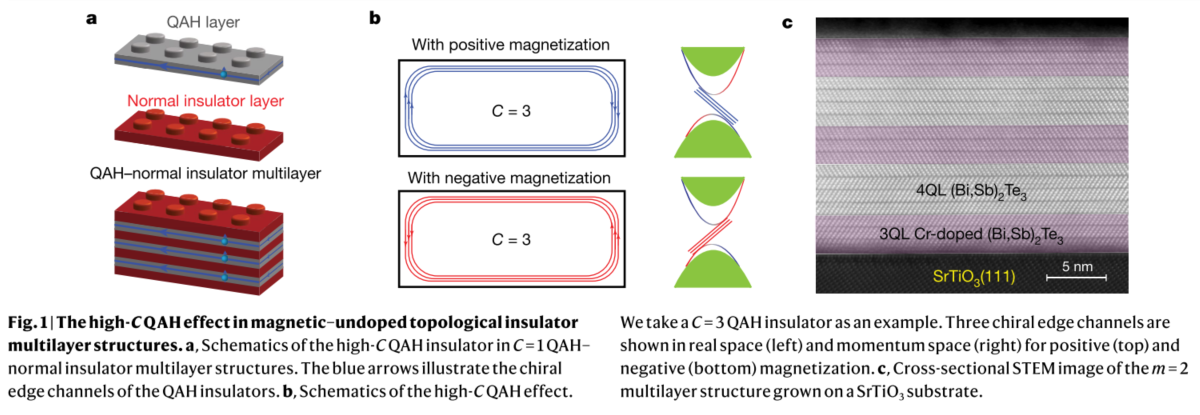
\includegraphics[scale=0.5]{pic/p19.png}
\end{figure}
\end{frame}
%================================================================
\section{Futher....}
\begin{frame}
\frametitle{Twisted}
\begin{itemize}
	\item arXiv:2012.07860v1(Magic angles and current-induced topology in twisted nodal superconductors)\\
	\item arXiv:2012.03986v1(Chiral $p$-wave superconductivity in a twisted array of proximitized quantum wires)
\end{itemize}
\begin{figure}
\centering
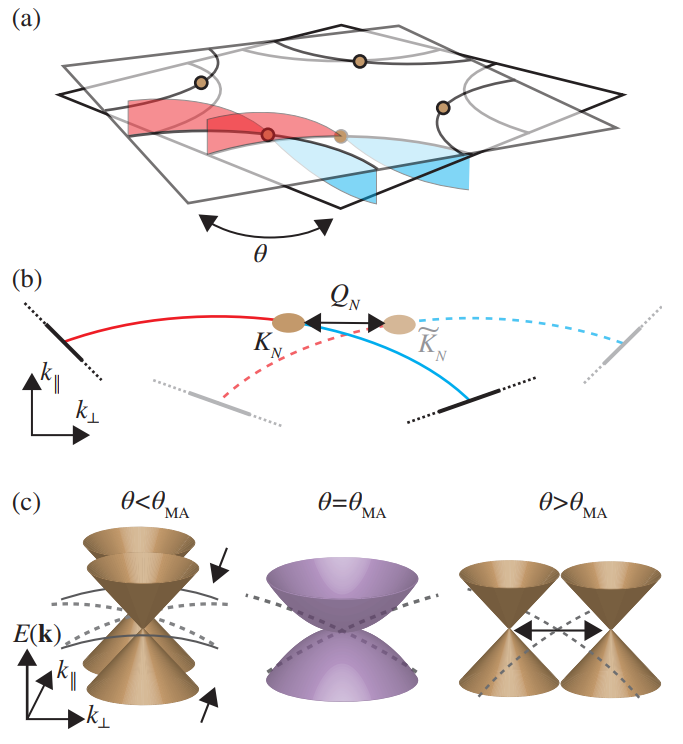
\includegraphics[scale=0.3]{pic/p20.png}
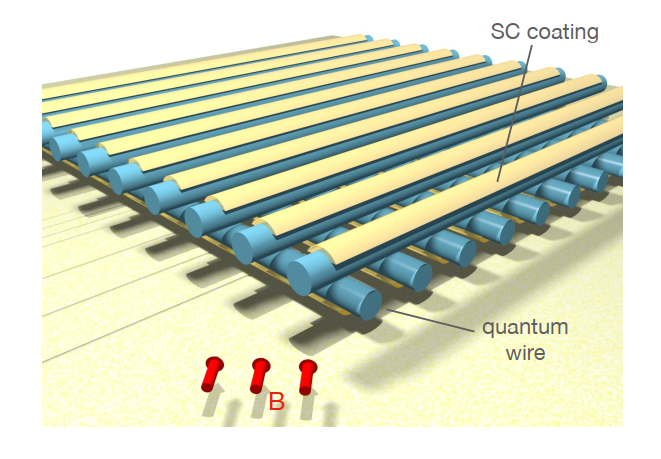
\includegraphics[scale=0.5]{pic/p21.png}
\end{figure}
\end{frame}
























\end{document} 